\documentclass[11pt]{article}
\usepackage[utf8]{inputenc}
\usepackage[dvips]{graphicx}
\usepackage{graphicx}
\usepackage{fancybox}
\usepackage{verbatim}
\usepackage{array}
\usepackage{latexsym}
\usepackage{alltt}
\usepackage{hyperref}
\usepackage{textcomp}
\usepackage{color}
\usepackage{amsmath}
\usepackage{amsfonts}
\usepackage{tikz}
\usepackage{float}
\usepackage{pdfpages}
\usepackage[most]{tcolorbox}
\usepackage[hmargin=3cm,vmargin=5.0cm]{geometry}
\usepackage{centernot}
\usepackage[table,xcdraw]{xcolor}
\usepackage{wrapfig}
\usepackage{minted}
\usepackage{listings}
\usepackage{algorithm}
\usepackage[noend]{algpseudocode}
%\topmargin=0cm
\topmargin=-2cm
\addtolength{\textheight}{6.5cm}
\addtolength{\textwidth}{2.0cm}
%\setlength{\leftmargin}{-5cm}
\setlength{\oddsidemargin}{0.0cm}
\setlength{\evensidemargin}{0.0cm}

\newtcolorbox{mybox}[3][breakable]
{
  colframe = #2!25,
  colback  = #2!10,
  coltitle = #2!20!black,  
  title    = {#3},
  #1,
}

\newenvironment{example}[1][\unskip]{\begin{mybox}{green}{\textbf{Example} {#1}}}{\end{mybox}}
\newenvironment{definition}[1]{\begin{mybox}{blue}{\textbf{Definition #1}}}{\end{mybox}}
\newenvironment{theorem}[1]{\begin{mybox}{red}{\textbf{Theorem #1}}}{\end{mybox}}

\title{CENG223 - Chapter 10: Graphs}
\author{Burak Metehan Tunçel}
\date{January 2022}

\begin{document}

\maketitle

\section{Graphs and Graph Models}

\begin{definition}{1}
A graph $G = (V,\ E)$ consists of $V$, a nonempty set of \textit{vertices} (or \textit{nodes}) and $E$, a set of \textit{edges}. Each edge has either one or two vertices associated with it, called its \textit{endpoints}. An edge is said to \textit{connect} its endpoints.
\end{definition}

\textbf{Remark} The set of vertices $V$ of a graph $G$ may be infinite. \textit{A graph with an infinite vertex set or an infinite number of edges is called an \textbf{infinite graph}}, and in comparison, \textit{a graph with a finite vertex set and a finite edge set is called a \textbf{finite graph}}. 

A graph in which each edge connects two different vertices and where
no two edges connect the same pair of vertices is called a \textbf{simple graph}. Note that in a simple graph, each edge is associated to an unordered pair of vertices, and no other edge is associated to this same edge. Consequently, when there is an edge of a simple graph associated to $\{u, v\}$, we can also say, without possible confusion, that $\{u, v\}$ is an edge of the graph.

Graphs that may have \textbf{multiple edges} connecting the same vertices are called \textbf{multigraphs}. When there are $m$ different edges associated to the same unordered pair of vertices $\{u, v\}$, we also say that $\{u, v\}$ is an edge of multiplicity $m$. That is, we can think of this set of edges as $m$ different copies of an edge $\{u, v\}$.

Edges that connect a vertex to itself are called \textbf{loops}, and sometimes we may even have more than one loop at a vertex. Graphs that may include loops, and possibly multiple edges connecting the same pair of vertices or a vertex to itself, are sometimes called \textbf{pseudographs}.

\begin{figure}[!h]
    \centering
    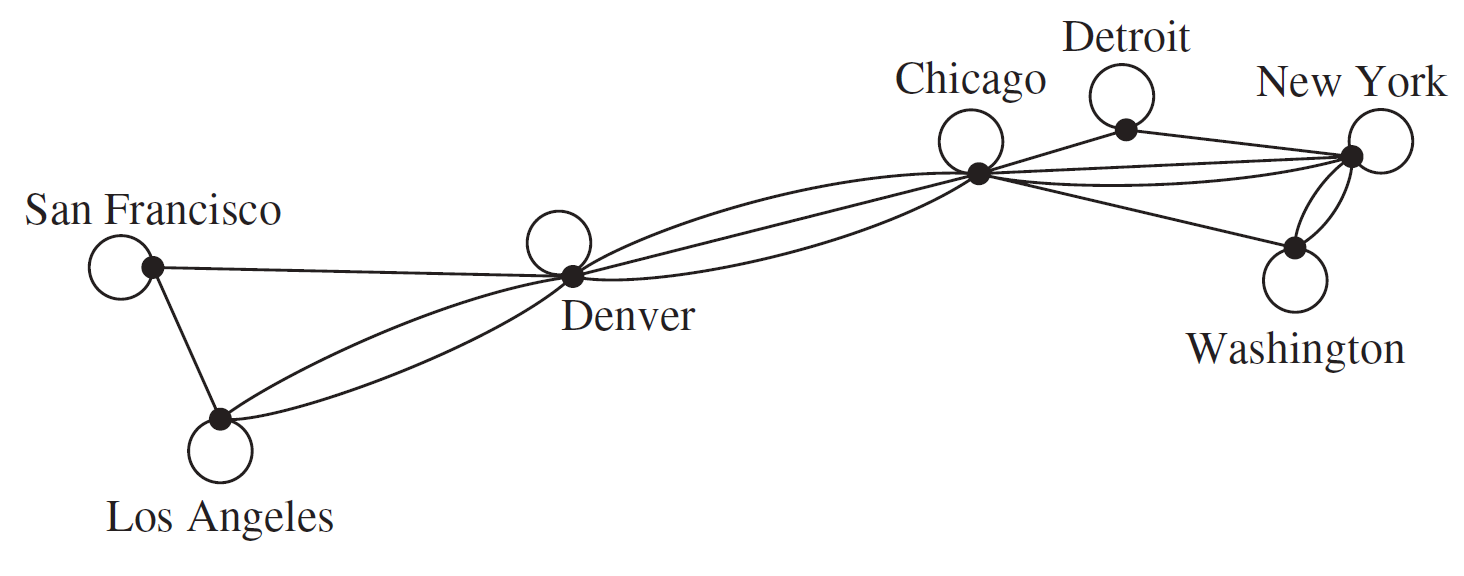
\includegraphics[width=0.75\textwidth]{img/ch10-figure3.png}
    \caption{A Graph}
    \label{fig:my_label}
\end{figure}


So far the graphs we have introduced are \textbf{undirected graphs}. Their edges are also said to be \textbf{undirected}. However, to construct a graph model, we may find it necessary to assign directions to the edges of a graph. Each edge of a directed graph is associated to an ordered pair. 

\begin{definition}{2}
A \textit{\textbf{directed graph}} (or \textit{\textbf{digraph}}) $(V,\ E)$ consists of a nonempty set of vertices $V$ and a set of \textit{directed edges} (or \textit{arcs}) $E$. Each directed edge is associated with an ordered pair of vertices. The directed edge associated with the ordered pair $(u,\ v)$ is said to \textit{start} at $u$ and \textit{end} at $v$.
\end{definition}

When a directed graph has no loops and has no multiple directed edges, it is called a \textbf{simple directed graph}. Because a simple directed graph has at most one edge associated to each ordered pair of vertices $(u,\ v)$, we call $(u,\ v)$ an edge if there is an edge associated to it in the graph.

Directed graphs that may have \textbf{multiple directed edges} from a vertex to a second (possibly the same) vertex are also used. We called such graphs \textbf{directed multigraphs}. When there are $m$ directed edges, each associated to an ordered pair of vertices $(u,\ v)$, we say that $(u,\ v)$ is an edge of multiplicity $m$.

For some models we may need a graph where some edges are undirected, while others are directed.A graph with \textit{both directed and undirected edges} is called a \textbf{mixed graph}. 

\begin{figure}[h!]
    \centering
    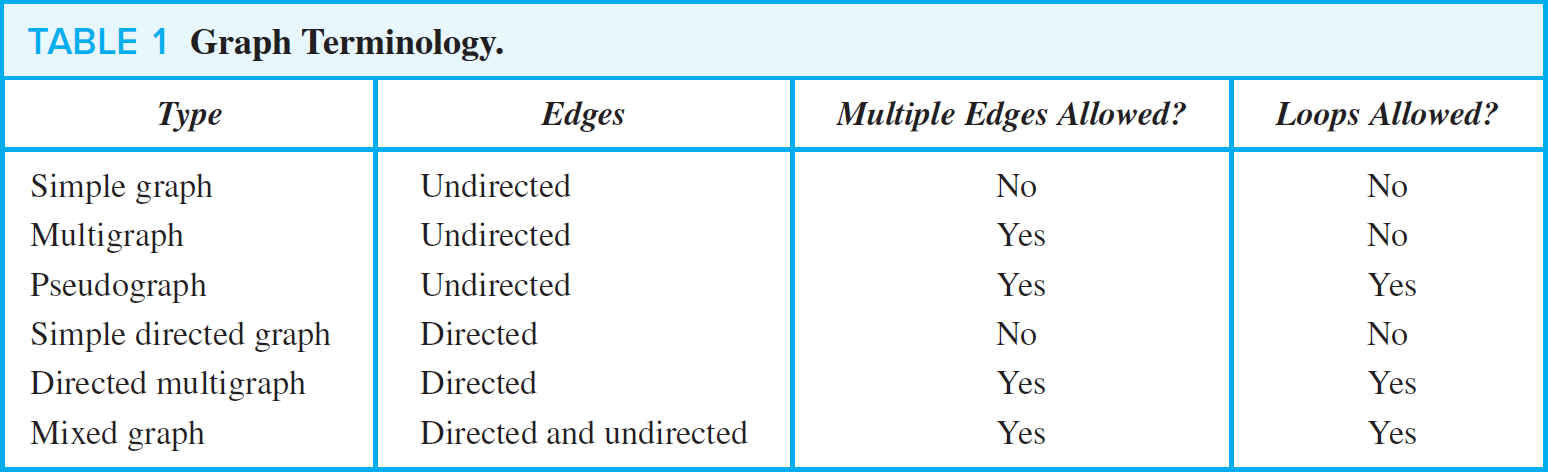
\includegraphics[width=\textwidth]{img/ch10-table1.png}
    \label{fig:my_label}
\end{figure}

This terminology for the various types of graphs is summarized in Table 1. We will sometimes use the term \textbf{graph} as a general term to describe graphs with directed or undirected edges (or both), with or without loops, and with or without multiple edges. At other times, when the context is clear, we will use the term graph to refer only to undirected graphs.

\subsection{Graph Models}

\textit{(It is better idea to read this part from the text book.)}


\section{Graph Terminology and Special Types of Graphs}

\subsection{Basic Terminology}

\begin{definition}{1}
Two vertices $u$ and $v$ in an undirected graph $G$ are called \textit{\textbf{adjacent}} (or \textit{neighbors}) in $G$ if $u$ and $v$ are endpoints of an edge $e$ of $G$. Such an edge $e$ is called \textit{\textbf{incident}} with the vertices $u$ and $v$ and $e$ is said to \textit{connect} $u$ and $v$.
\end{definition}

\begin{definition}{2}
The set of all neighbors of a vertex $v$ of $G = (V,\ E)$, denoted by $N(v)$, is called the \textit{\textbf{neighborhood}} of $v$. If $A$ is a subset of $V$, we denote by $N(A)$ the set of all vertices in $G$ that are adjacent to at least one vertex in $A$. So, $N(A) = \bigcup_{v \in A} N(v)$.
\end{definition}

\begin{definition}{3}
The \textit{\textbf{degree} of a vertex in an undirected graph} is the number of edges incident with it, except that a loop at a vertex contributes twice to the degree of that vertex. The degree of the vertex $v$ is denoted by deg($v$).
\end{definition}

A vertex of degree zero is called \textbf{isolated}. It follows that an isolated vertex is not adjacent to any vertex. A vertex is \textbf{pendant} if and only
if it has degree one. Consequently, a pendant vertex is adjacent to exactly one other vertex. Examining the degrees of vertices in a graph model can provide useful information about the model.

What do we get when we add the degrees of all the vertices of a graph $G = (V,\ E)$? \textit{Each edge contributes two to the sum of the degrees of the vertices} because an edge is incident with exactly two (possibly equal) vertices. This means that \textit{\textbf{the sum of the degrees of the vertices is twice the number of edges}}. We have the result in Theorem 1, which is sometimes called the \textit{\textbf{handshaking theorem}} (and is also often known as the \textit{\textbf{handshaking lemma}}).

\begin{theorem}{1: The Handshaking Theorem}
Let $G = (V,\ E)$ be an undirected graph with $m$ edges. Then
\begin{align*}
    &2m = \sum_{v \in V} deg(v)& & & & & &
\end{align*}

(Note that this applies even if multiple edges and loops are present.)
\end{theorem}

Theorem 1 shows that the sum of the degrees of the vertices of an undirected graph is even. This simple fact has many consequences, one of which is given as Theorem 2.

\begin{theorem}{2}
An undirected graph has an even number of vertices of odd degree.
\end{theorem}

\textbf{Proof:} Let $V_1$ and $V_2$ be the set of vertices of even degree and the set of vertices of odd degree, respectively, in an undirected graph $G = (V,\ E)$ with $m$ edges. Then

\begin{align*}
    2m = \sum_{v \in V} deg(v) = \sum_{v \in V_1} deg(v) + \sum_{v \in V_2} deg(v)& & & &    
\end{align*}

Because $deg(v)$ is even for $v \in V_1$, the first term in the right-hand side of the last equality is even. Furthermore, the sum of the two terms on the right-hand side of the last equality is even, because this sum is $2m$. Hence, the second term in the sum is also even. Because all the terms in this sum are odd, there must be an even number of such terms. Thus, there are an even number of vertices of odd degree.

Terminology for graphs with directed edges reflects the fact that edges in directed graphs have directions.

\begin{definition}{4}
When $(u,\ v)$ is an edge of the graph $G$ with directed edges, $u$ is said to be \textit{adjacent to $v$} and $v$ is said to be \textit{adjacent from $u$}. The vertex $u$ is called the \textit{initial vertex} of $(u,\ v)$, and $v$ is called the \textit{terminal} or \textit{end} vertex of $(u,\ v)$. The initial vertex and terminal vertex of a loop are the same.
\end{definition}

Because the edges in graphs with directed edges are ordered pairs, the definition of the degree of a vertex can be refined to reflect the number of edges with this vertex as the initial vertex and as the terminal vertex.

\begin{definition}{5}
In a graph with directed edges the \textit{in-degree of a vertex $v$}, denoted by $deg^-(v)$, is the number of edges with $v$ as their \textit{terminal vertex}. The \textit{out-degree of $v$}, denoted by $deg^+(v)$, is the number of edges with $v$ as their \textit{initial vertex}.\\
(Note that a loop at a vertex contributes 1 to both the in-degree and the out-degree of this vertex.)
\end{definition}

Because each edge has an initial vertex and a terminal vertex, the sum of the in-degrees and the sum of the out-degrees of all vertices in a graph with directed edges are the same. Both of these sums are the number of edges in the graph. This result is stated as Theorem 3.

\begin{theorem}{3}
Let $G = (V,\ E)$ be a graph with directed edges. Then
\begin{align*}
    &\sum_{v \in V} deg^-(v) = \sum_{v \in V} deg^+(v) = |E| & & & & &
\end{align*}
\end{theorem}

There are many properties of a graph with directed edges that do not depend on the direction of its edges. Consequently, it is often useful to ignore these directions. The undirected graph that results from ignoring directions of edges is called the \textbf{underlying undirected graph}. A graph with directed edges and its underlying undirected graph have the same number of edges.

\subsection{Some Special Simple Graphs}

\subsubsection{Complete Graphs}
\setcounter{figure}{2}
A \textbf{complete graph on $n$ vertices}, denoted by $K_n$, is a simple graph that contains exactly one edge between each pair of distinct vertices. The graphs $K_n$, for $n = 1, 2, 3, 4, 5, 6$, are displayed in Figure 3. A simple graph for which there is at least one pair
of distinct vertex not connected by an edge is called noncomplete.

\begin{figure}[h!]
    \centering
    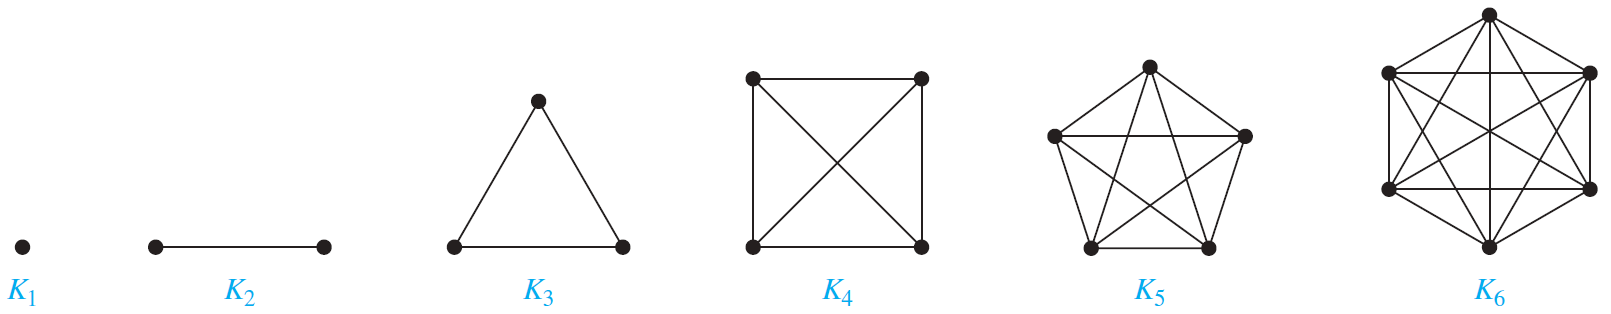
\includegraphics[width=\textwidth]{img/ch10.2-figure3.png}
    \caption{The graphs $K_n$ for $1 \leq n \leq 6$.}
    \label{fig:my_label}
\end{figure}

\subsubsection{Cycles}

A \textbf{cycle} $C_n$, $n \geq 3$, consists of $n$ vertices $v_1, v_2, ..., v_n$ and edges $\{v_1,\ v_2\},\ \{v_2,\ v_3\},\ ...,\ \{v_{n-1},\ v_n\}$, and $\{v_n,\ v_1\}$. The cycles $C_3,\ C_4,\ C_5$, and $C_6$ are displayed in Figure 4.

\begin{figure}[h!]
    \centering
    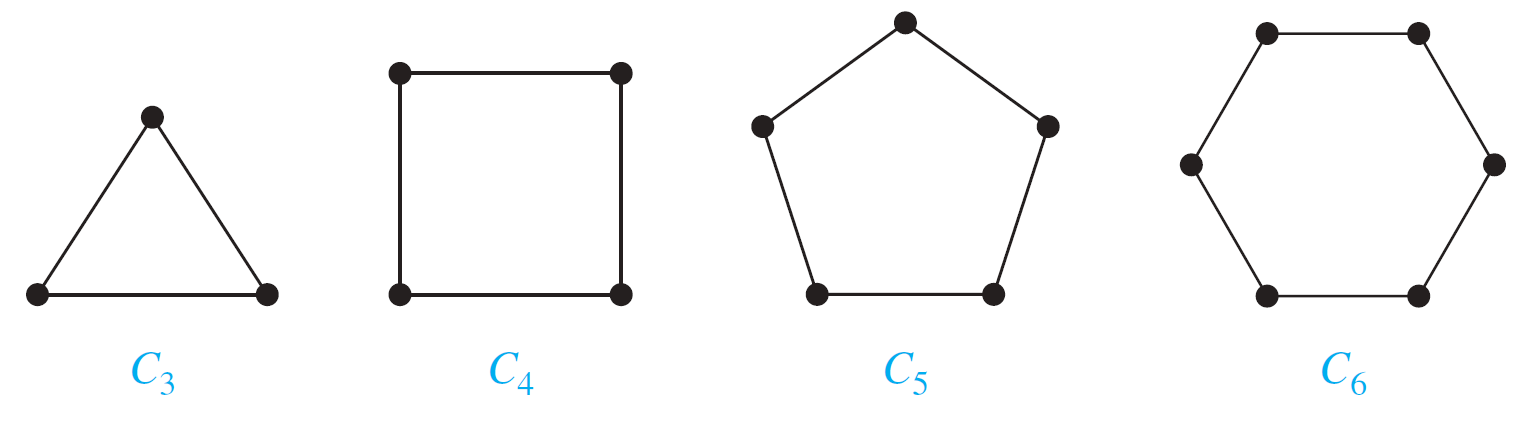
\includegraphics[width=.75\textwidth]{img/ch10.2-figure4.png}
    \caption{The cycles $C_3,\ C_4,\ C_5$, and $C_6$.}
    \label{fig:my_label}
\end{figure}

\subsubsection{Wheels}

We obtain a \textbf{wheel} $W_n$ when we add an additional vertex to a cycle $C_n$, for $n \geq 3$, and connect this new vertex to each of the $n$ vertices in $C_n$, by new edges. The wheels $W_3,\ W_4,\ W_5$, and $W_6$ are displayed in Figure 5.

\begin{figure}[h!]
    \centering
    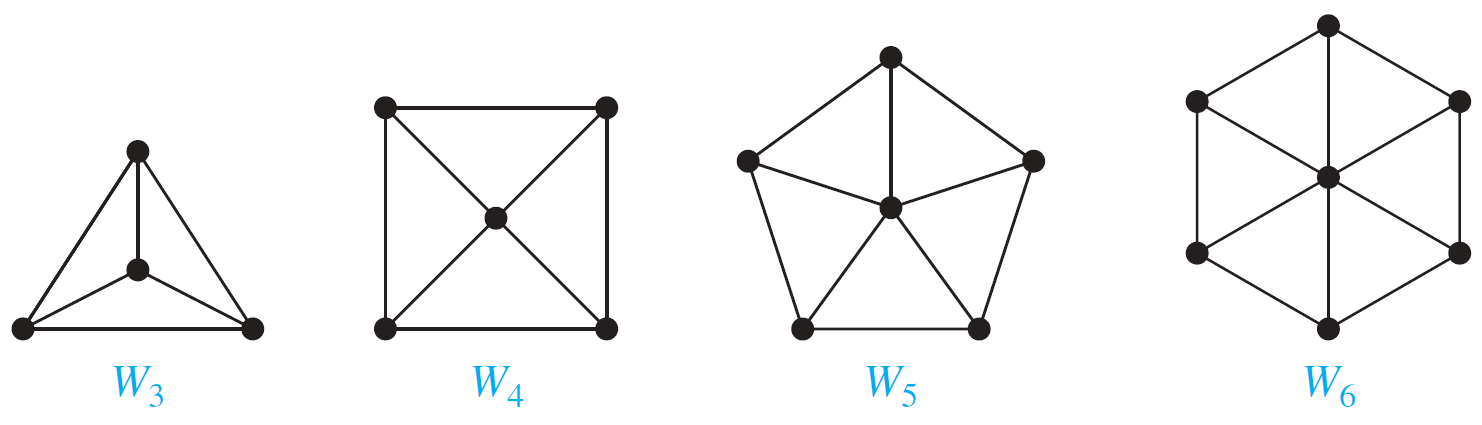
\includegraphics[width=.75\textwidth]{img/ch10.2-figure5.png}
    \caption{The wheels $W_3,\ W_4,\ W_5$, and $W_6$.}
    \label{fig:my_label}
\end{figure}

\subsubsection{$n$-Cubes}

An \textbf{$n$-dimensional hypercube}, or \textbf{$n$-cube}, denoted by $Q_n$, is a graph that has vertices representing the $2^n$ bit strings of length $n$. Two vertices are adjacent if and only if the bit strings that they represent differ in exactly one bit position. We display $Q_1,\ Q_2$, and $Q_3$ in Figure 6.

\begin{figure}[h!]
    \centering
    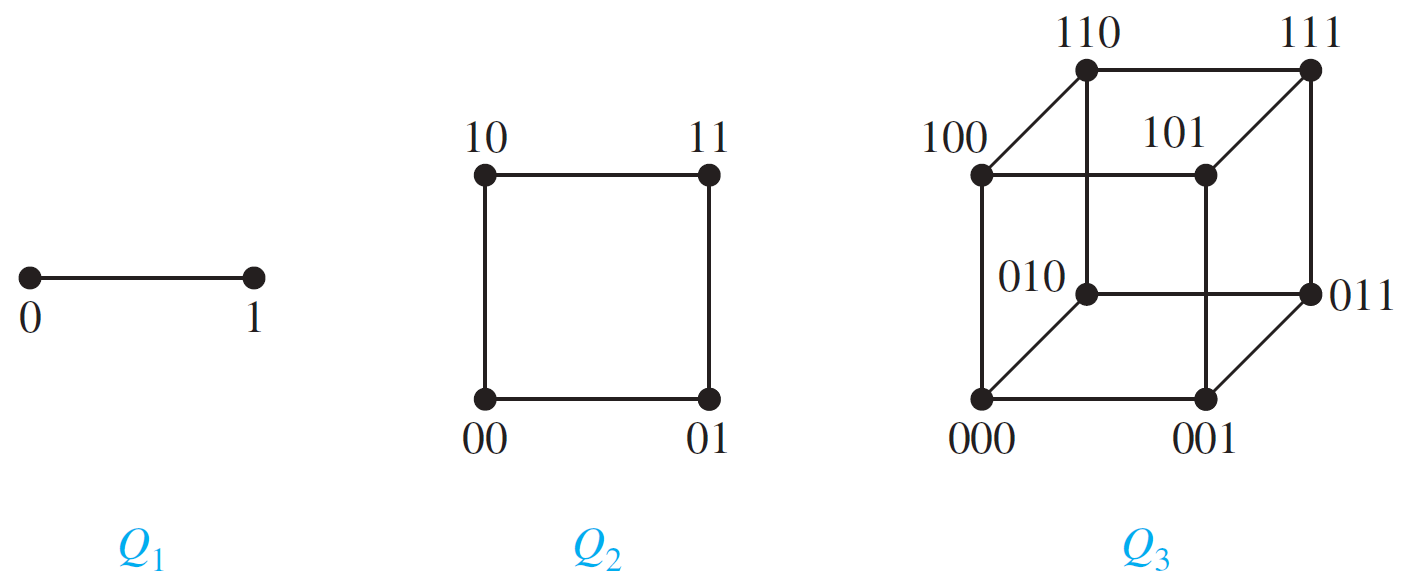
\includegraphics[width=.6\textwidth]{img/ch10.2-figure6.png}
    \caption{The $n$-cube $Q_n$, $n = 1, 2, 3$.}
    \label{fig:my_label}
\end{figure}

\subsection{Bipartite Graphs}

Sometimes a graph has the property that its vertex set can be divided into two disjoint subsets such that each edge connects a vertex in one of these subsets to a vertex in the other subset. For example, consider the graph representing marriages between men and women in a village, where each person is represented by a vertex and a marriage is represented by an edge. In this graph, each edge connects a vertex in the subset of vertices representing males and a vertex in the subset of vertices representing females. This leads us to Definition 6.

\begin{definition}{6}
A simple graph $G$ is called \textit{\textbf{bipartite}} if its vertex set $V$ can be partitioned into two disjoint sets $V_1$ and $V_2$ such that every edge in the graph connects a vertex in $V_1$ and a vertex in $V_2$ (so that no edge in $G$ connects either two vertices in $V_1$ or two vertices in $V_2$). When this condition holds, we call the pair $(V1,\ V2)$ a \textit{\textbf{bipartition} of the vertex set $V$ of $G$}.
\end{definition}

Theorem 4 provides a useful criterion for determining whether a graph is bipartite.

\begin{theorem}{4}
A simple graph is bipartite if and only if it is possible to assign one of two different colors to each vertex of the graph so that no two adjacent vertices are assigned the same color.
\end{theorem}

\textbf{Proof:} First, suppose that $G = (V,\ E)$ is a bipartite simple graph. Then $V = V_1 \cup V_2$, where $V_1$ and $V_2$ are disjoint sets and every edge in $E$ connects a vertex in $V_1$ and a vertex in $V_2$. If we assign one color to each vertex in $V_1$ and a second color to each vertex in $V_2$, then no two
adjacent vertices are assigned the same color.

Now suppose that it is possible to assign colors to the vertices of the graph using just two colors so that no two adjacent vertices are assigned the same color. Let $V_1$ be the set of vertices assigned one color and $V_2$ be the set of vertices assigned the other color. Then, $V_1$ and $V_2$ are disjoint and $V = V_1 \cup V_2$. Furthermore, every edge connects a vertex in $V_1$ and a vertex in $V_2$ because no two adjacent vertices are either both in $V_1$ or both in $V_2$. Consequently, $G$ is bipartite.

\subsubsection{Complete Bipartite Graphs}

A \textbf{complete bipartite graph $K_{m,n}$} is a graph that has its vertex
set partitioned into two subsets of $m$ and $n$ vertices, respectively with an edge between two vertices if and only if one vertex is in the first subset and the other vertex is in the second subset. The complete bipartite graphs $K_{2,3}$, $K_{3,3}$, $K_{3,5}$, and $K_{2,6}$ are displayed in Figure 9.

\setcounter{figure}{8}
\begin{figure}[h!]
    \centering
    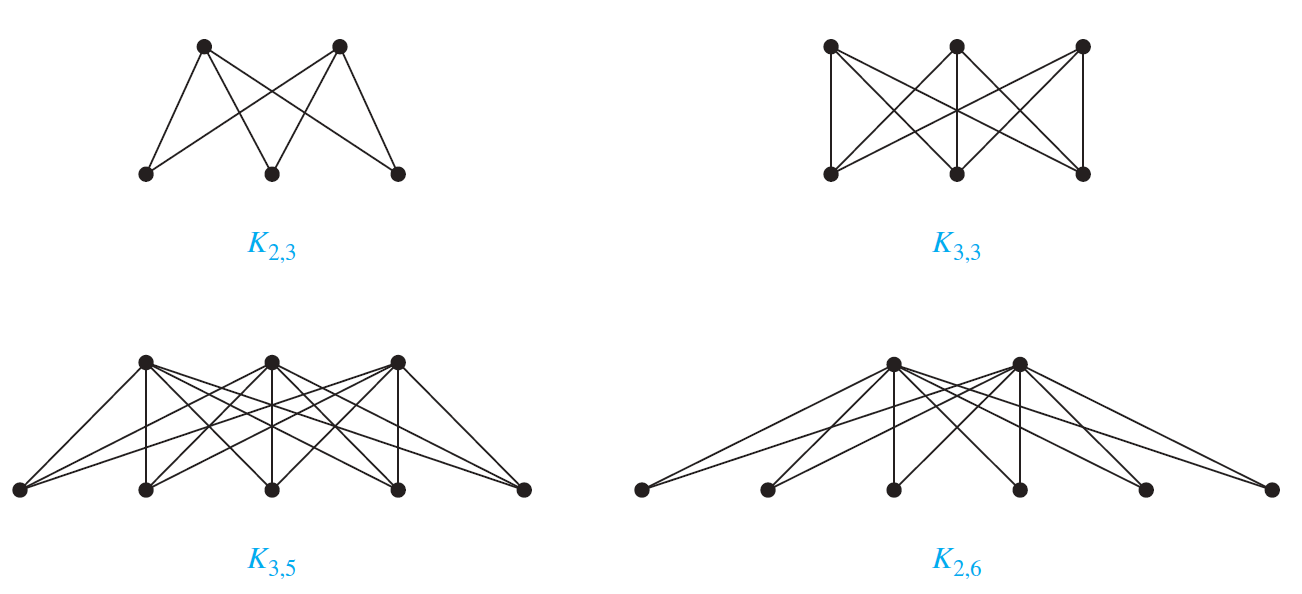
\includegraphics[width=.6\textwidth]{img/ch10.2-figure9.png}
    \caption{Some complete bipartite graphs.}
    \label{fig:my_label}
\end{figure}

\subsection{Bipartite Graphs and Matchings}

Finding an assignment of jobs to employees can be thought of as finding a matching in the graph model, where a \textbf{matching} $M$ in a simple graph $G = (V,\ E)$ is a subset of the set $E$ of edges of the graph such that no two edges are incident with the same vertex. In other words, a matching is a subset of edges such that if $\{s,\ t\}$ and $\{u,\ v\}$ are distinct edges of the matching, then $s$, $t$, $u$, and $v$ are distinct. A vertex that is the endpoint of an edge of a matching $M$ is said to be \textbf{matched} in $M$; otherwise, it is said to be \textbf{unmatched}. A \textbf{maximum matching} is a matching with the largest number of edges. 

We say that a matching $M$ in a bipartite graph $G = (V,\ E)$ with bipartition $(V_1,\ V_2)$ is a \textbf{complete matching from $V_1$ to $V_2$} if every vertex in $V_1$ is the endpoint of an edge in the matching, or equivalently, if $|M| = |V_1|$. For example, to assign jobs to employees so that the largest number of jobs are assigned employees, we seek a maximum matching in the graph that models employee capabilities. To assign employees to all jobs we seek a complete matching from the set of jobs to the set of employees.

\subsubsection{Necessary and Sufficient Conditions for Complete Matchings}

We now turn our attention to the question of determining whether a complete matching from $V_1$ to $V_2$ exists when $(V_1,\ V_2)$ is a bipartition of a bipartite graph $G = (V,\ E)$. We will introduce a theorem that provides a set of \textit{necessary} and \textit{sufficient} conditions for the existence of a complete matching. This theorem was proved by Philip Hall in 1935.

\begin{theorem}{5: Hall's Marriage Theorem}
The bipartite graph $G = (V,\ E)$ with bipartition $(V_1,\ V_2)$ has a complete matching from $V_1$ to $V_2$ if and only if $|N(A)| \geq |A|$ for all subsets $A$ of $V_1$.
\end{theorem}

\textbf{Proof:} \textit{(It is better to read the Proof from text book).}

\subsection{Some Applications of Special Types of Graphs}

\textit{(It is better idea to read this part from the text book.)}

\subsection{New Graphs from Old}

When edges and vertices are removed from a graph, without removing endpoints of any remaining edges, a smaller graph is obtained. Such a graph is called a \textbf{subgraph} of the original graph.

\begin{definition}{7}
A \textit{\textbf{subgraph} of a graph $G = (V,\ E)$} is a graph $H = (W,\ F)$, where $W \subseteq V$ and $F \subseteq E$. A subgraph $H$ of $G$ is a \textit{proper subgraph} of $G$ if $H \neq G$.
\end{definition}

Given a set of vertices of a graph, we can form a subgraph of this graph with these vertices and the edges of the graph that connect them.

\begin{definition}{8}
Let $G = (V,\ E)$ be a simple graph. The \textbf{subgraph induced} by a subset $W$ of the vertex set $V$ is the graph $(W,\ F)$, where the edge set $F$ contains an edge in $E$ if and only if both endpoints of this edge are in $W$.
\end{definition}

\subsubsection{Removing or Adding Edges of a Graph} 

Given a graph $G = (V,\ E)$ and an edge $e \in E$, we can produce a subgraph of $G$ by removing the edge $e$. The resulting subgraph, denoted by $G - e$, has the same vertex set $V$ as $G$. Its edge set is $E - \{e\}$. Hence,

$G - e = (V,\ E - \{e\})$.

\noindent Similarly, if $E^{'}$ is a subset of $E$, we can produce a subgraph of $G$ by removing the edges in $E^{'}$ from the graph. The resulting subgraph has the same vertex set $V$ as $G$. Its edge set is $E - E^{'}$.

We can also add an edge $e$ to a graph to produce a new larger graph when this edge connects two vertices already in $G$. We denote by $G + e$ the new graph produced by adding a new edge $e$, connecting two previously nonincident vertices, to the graph $G$. Hence,

$G + e = (V,\ E \cup \{e\})$.

\noindent The vertex set of $G + e$ is the same as the vertex set of $G$ and the edge set is the union of the edge set of $G$ and the set $\{e\}$.

\subsubsection{Edge Contractions}

Sometimes when we remove an edge from a graph, we do not want to retain the endpoints of this edge as separate vertices in the resulting subgraph. In such a case we perform an \textbf{edge contraction}, which removes an edge $e$ with endpoints $u$ and $v$ and merges $u$ and $w$ into a new single vertex $w$, and for each edge with $u$ or $v$ as an endpoint replaces the edge with one with $w$ as endpoint in place of $u$ or $v$ and with the same second endpoint. 
Hence, the contraction of the edge $e$ with endpoints $u$ and $v$ in the graph $G = (V,\ E)$ produces a new graph $G^{'} = (V^{'},\ E^{'})$ (which is not a subgraph of G), where $V^{'} = V - \{u,\ v\} \cup \{w\}$ and $E^{'}$ contains the edges in $E$ which do not have either $u$ or $v$ as endpoints and an edge connecting $w$ to every neighbor of either $u$ or $v$ in $V$. For example, the contraction of the edge connecting the vertices $e$ and $c$ in the graph $G_1$ in Figure 16 produces a new graph $G^{'}_1$ with vertices $a$, $b$, $d$, and $w$. As in $G_1$, there is an edge in $G^{'}_1$ connecting $a$ and $b$ and an edge connecting $a$ and $d$. There also is an edge in $G^{'}_1$ that connects $b$ and $w$ that replaces the edges connecting $b$ and $c$ and connecting $b$ and $e$ in $G_1$ and an edge in $G^{'}_1$ that connects $d$ and $w$ replacing the edge connecting $d$ and $e$ in $G_1$.

\setcounter{figure}{15}
\begin{figure}[h!]
    \centering
    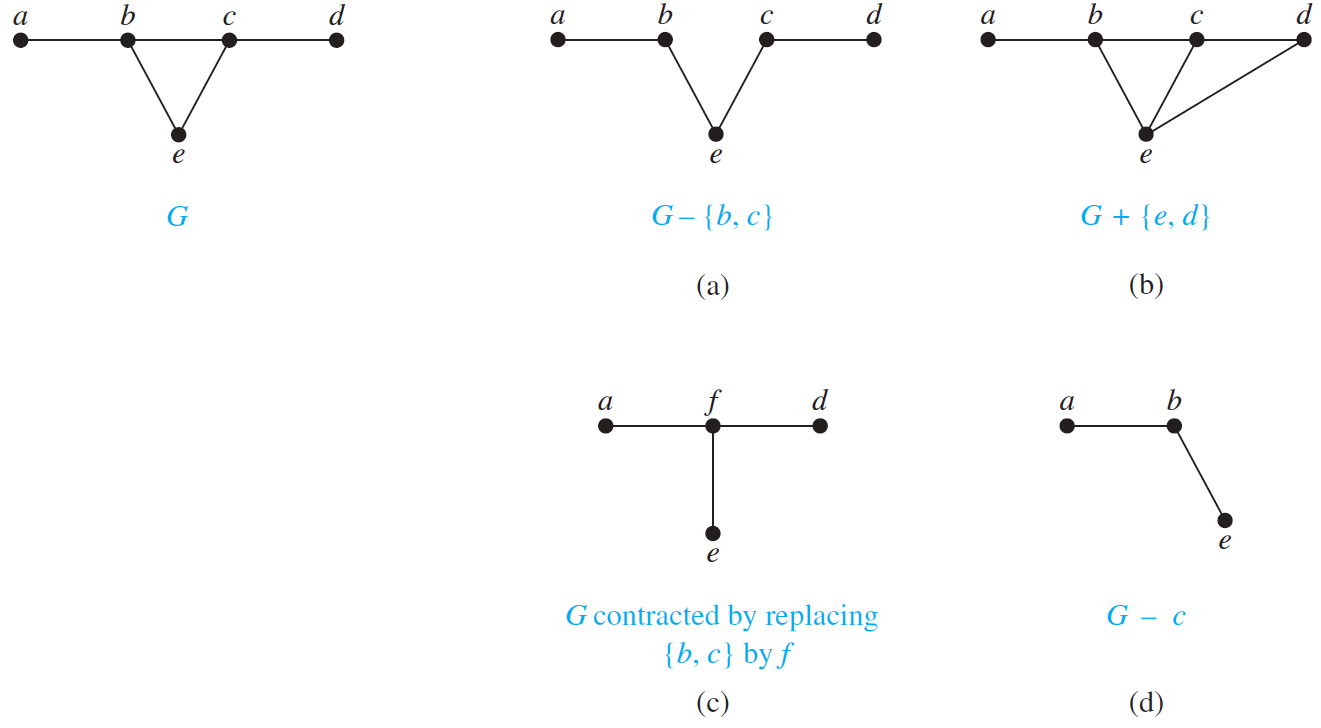
\includegraphics[width=\textwidth]{img/ch10.2-figure16.png}
    \caption{The graph $G$ and four graphs resulting from different operations on $G$}
    \label{fig:my_label}
\end{figure}

\subsubsection{Removing Vertices From a Graph}

When we remove a vertex $v$ and all edges incident to it from $G = (V,\ E)$, we produce a subgraph, denoted by $G - v$. Observe that $G - v = (V - \{v\},\ E^{'})$, where $E^{'}$ is the set of edges of $G$ not incident to $v$. Similarly, if $V^{'}$ is a subset of $V$, then the graph $G - V^{'}$ is the subgraph $(V - V^{'},\ E^{'})$, where $E^{'}$ is the set of edges of $G$ not incident to a vertex in $V^{'}$.

\subsubsection{Graph Unions}

Two or more graphs can be combined in various ways. The new graph that contains all the vertices and edges of these graphs is called the \textbf{union} of the graphs. We will give a more formal definition for the union of two simple graphs.

\begin{definition}{9}
The \textit{union} of two simple graphs $G_1 = (V_1,\ E_1)$ and $G_2 = (V_2,\ E_2)$ is the simple graph with vertex set $V_1 \cup V_2$ and edge set $E_1 \cup E_2$. The union of $G_1$ and $G_2$ is denoted by $G_1 \cup G_2$.
\end{definition}


\section{Representing Graphs and Graph Isomorphism}

\subsection{Introduction}

There are many useful ways to represent graphs. As we will see throughout this chapter, in working with a graph it is helpful to be able to choose its most convenient representation. In this section we will show how to represent graphs in several different ways.

Sometimes, two graphs have exactly the same form, in the sense that there is a one-to-one correspondence between their vertex sets that preserves edges. In such a case, we say that the two graphs are \textbf{isomorphic}. Determining whether two graphs are isomorphic is an important problem of graph theory that we will study in this section.

\subsection{Representing Graphs}

One way to represent a graph without multiple edges is to list all the edges of this graph. Another way to represent a graph with no multiple edges is to use \textbf{adjacency lists}, which specify the vertices that are adjacent to each vertex of the graph.

\begin{figure}[h!]
    \centering
    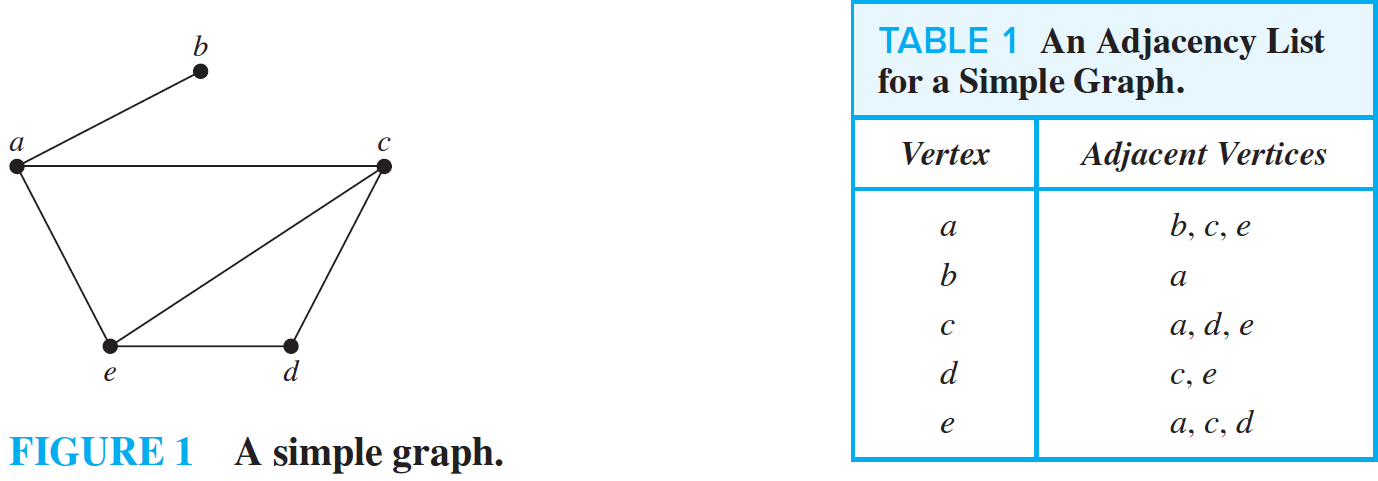
\includegraphics[width=.7\textwidth]{img/ch10.3-figure1.png}
    \label{fig:my_label}
\end{figure}

\subsection{Adjacency Matrices}

Carrying out graph algorithms using the representation of graphs by lists of edges, or by adjacency lists, can be cumbersome if there are many edges in the graph. To simplify computation, graphs can be represented using matrices. Two types of matrices commonly used to represent graphs will be presented here. One is based on the adjacency of vertices, and the other is based on incidence of vertices and edges.

Suppose that $G = (V,\ E)$ is a simple graph where $|V| = n$. Suppose that the vertices of $G$ are listed arbitrarily as $v_1, v_2, ..., v_n$. The \textbf{adjacency matrix $\mathbf{A}$} (or $\mathbf{A}_G$) of $G$, with respect to this listing of the vertices, is the $n \times n$ zero-one matrix with 1 as its $(i, j)^{th}$ entry when $v_i$ and $v_j$ are adjacent, and 0 as its $(i, j)^{th}$ entry when they are not adjacent. In other words, if its adjacency
matrix is $A = [a_{ij}]$, then

$a_{ij} = 
    \begin{cases}
        1& \text{if $\{v_i, v_j\}$ is an edge of $G$},\\
        0& \text{otherwise}.
    \end{cases}$

\begin{figure}[h!]
    \centering
    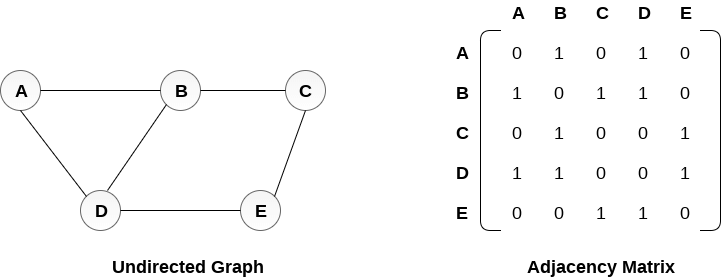
\includegraphics[width=.8\textwidth]{img/ch10.3-adjaceny_matrix.png}
    \label{fig:my_label}
\end{figure}

Note that an adjacency matrix of a graph is based on the ordering chosen for the vertices. Hence, there may be as many as $n!$ different adjacency matrices for a graph with $n$ vertices, because there are $n!$ different orderings of $n$ vertices.

The adjacency matrix of a simple graph is symmetric, that is, $a_{ij} = a_{ji}$, because both of these entries are 1 when $v_i$ and $v_j$ are adjacent, and both are 0 otherwise. Furthermore, because a simple graph has no loops, each entry $a_{ii}$, $i = 1, 2, 3, ..., n$, is 0.

Adjacency matrices can also be used to represent undirected graphs with loops and with multiple edges. A loop at the vertex $v_i$ is represented by a 1 at the $(i, i)^{th}$ position of the adjacency matrix. When multiple edges connecting the same pair of vertices $v_i$ and $v_j$, or multiple loops at the same vertex, are present, the adjacency matrix is no longer a zero-one matrix, because the $(i, j)^{th}$ entry of this matrix equals the number of edges that are associated to $\{v_i,\ v_j\}$. All undirected graphs, including multigraphs and pseudographs, have symmetric adjacency matrices.

\begin{figure}[h!]
\begin{minipage}[l]{0.4\textwidth}
    \centering
    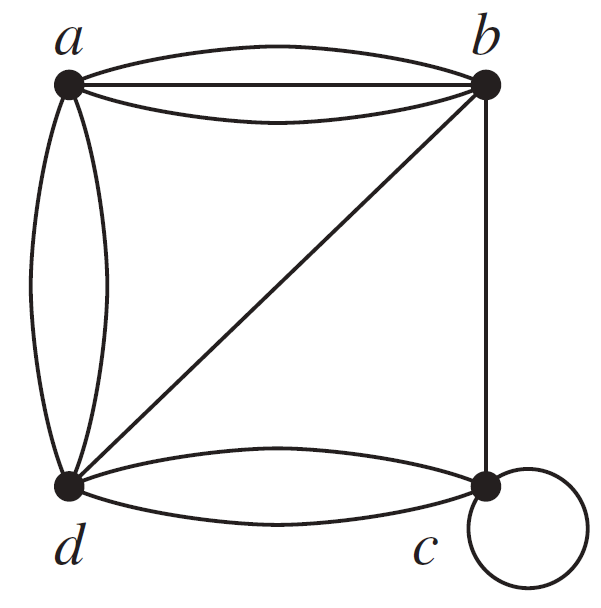
\includegraphics[width=\textwidth]{img/ch10.3-figure5_1.png}
\end{minipage}\hfill
\begin{minipage}[l]{0.4\textwidth}
    \centering
    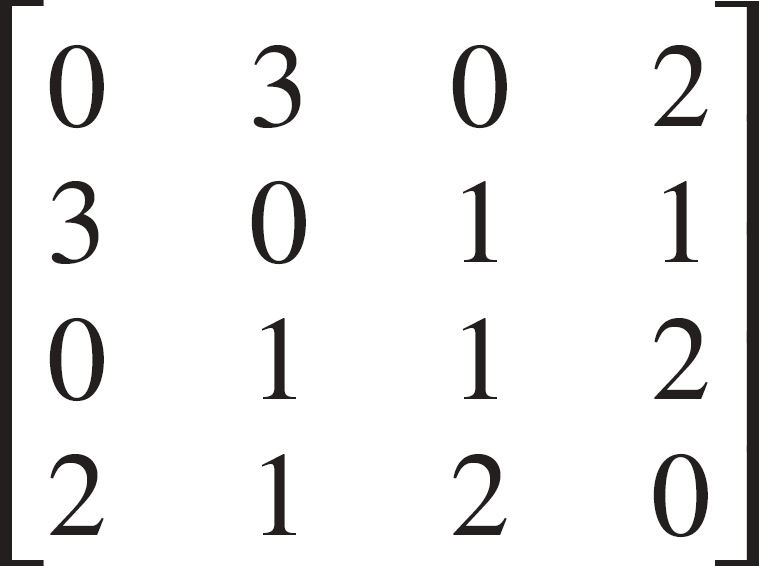
\includegraphics[width=\textwidth]{img/ch10.3-figure5_2.png}
\end{minipage}\hfill
\end{figure}

We used zero–one matrices to represent directed graphs. The matrix for a directed graph $G = (V,\ E)$ has a 1 in its $(i, j)^{th}$ position if there is an edge from $v_i$ to $v_j$, where $v_1, v_2, ..., v_n$ is an arbitrary listing of the vertices of the directed graph. In other words, if $A = [a_{ij}]$ is the adjacency matrix for the directed graph with respect to this listing of the vertices, then

$a_{ij} =
    \begin{cases}
        1 & \text{if $(v_i, v_j)$ is an edge of $G$},\\
        0 & \text{otherwise}
    \end{cases}$
    
\noindent The adjacency matrix for a directed graph does not have to be symmetric, because there may not be an edge from $v_j$ to $v_i$ when there is an edge from $v_i$ to $v_j$.

Adjacency matrices can also be used to represent directed multigraphs. Again, such matrices are not zero–one matrices when there are multiple edges in the same direction connecting two vertices. In the adjacency matrix for a directed multigraph, $a_{ij}$ equals the number of edges that are associated to $(v_i, v_j)$.

\subsubsection{Trade-Offs Between Adjacency Lists and Adjacency Matrices}

When a simple graph contains relatively few edges, that is, when it is \textbf{sparse}, it is usually preferable to use adjacency lists rather than an adjacency matrix to represent the graph. For example, if each vertex has degree not exceeding $c$, where $c$ is a constant \textit{much smaller} than $n$, then each adjacency list contains $c$ or fewer vertices. Hence, there are no more than $cn$ items in all these adjacency lists. On the other hand, the adjacency matrix for the graph has $n^2$ entries. Note, however, that the adjacency matrix of a sparse graph is a \textbf{sparse matrix}, that is, a matrix with few nonzero entries, and there are special techniques for representing, and computing with, sparse matrices.

Now suppose that a simple graph is \textbf{dense}, that is, suppose that it contains many edges, such as a graph that contains more than half of all possible edges. In this case, using an adjacency matrix to represent the graph is usually preferable over using adjacency lists. To see why, we compare the complexity of determining whether the possible edge $\{v_i, v_j\}$ is present. Using an adjacency matrix, we can determine whether this edge is present by examining the $(i, j)^{th}$ entry in the matrix. This entry is 1 if the graph contains this edge and is 0 otherwise. Consequently, we need make only one comparison, namely, comparing this entry with 0, to determine whether this edge is present. On the other hand, when we use adjacency lists to represent the graph, we need to search the list of vertices adjacent to either $v_i$ or $v_j$ to determine whether this edge is present. This can require $\Theta(|V|)$ comparisons when many edges are present.

\subsection{Incidence Matrices}

Another common way to represent graphs is to use \textbf{incidence matrices}. Let $G = (V,\ E)$ be an undirected graph. Suppose that $v_1, v_2, ..., v_n$ are the vertices and $e_1, e_2, ..., e_m$ are the edges of $G$. Then the incidence matrix with respect to this ordering of $V$ and $E$ is the $n \times m$ matrix
$\mathbf{M} = [m_{ij}]$, where

$m_{ij} =
\begin{cases}
    1 & \text{when edge $e_j$ is incident with $v_i$},\\
    0 & \text{otherwise}.
\end{cases}$

\begin{figure}[!h]
    \centering
    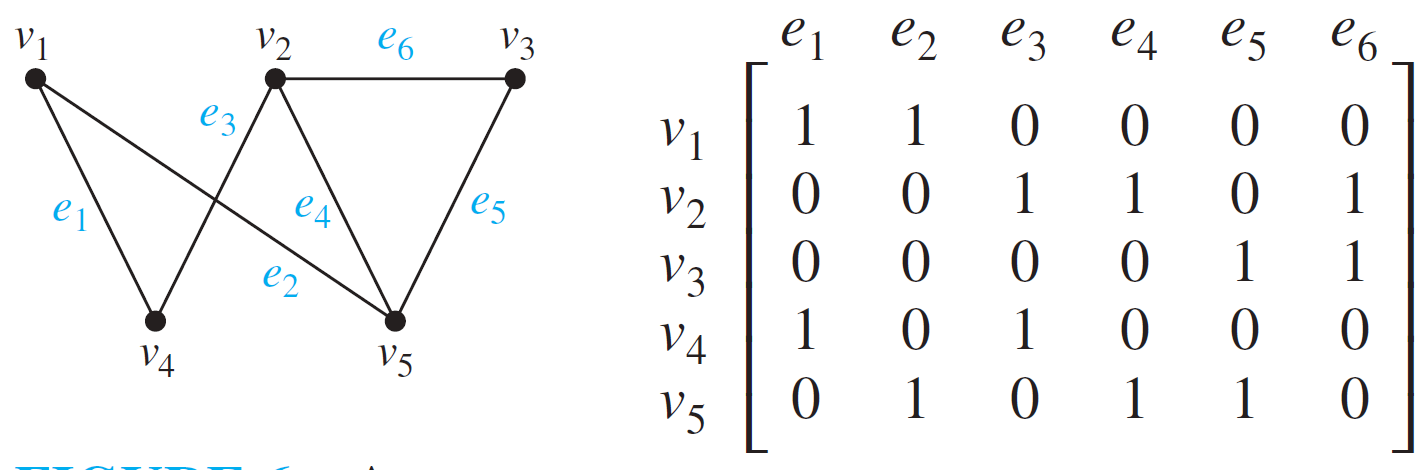
\includegraphics[width=.75\textwidth]{img/ch10.3-figure6.png}
    \label{fig:my_label}
\end{figure}

Incidence matrices can also be used to represent multiple edges and loops. Multiple edges are represented in the incidence matrix using columns with identical entries, because these edges are incident with the same pair of vertices. Loops are represented using a column with exactly one entry equal to 1, corresponding to the vertex that is incident with this loop.

\begin{figure}[!h]
    \centering
    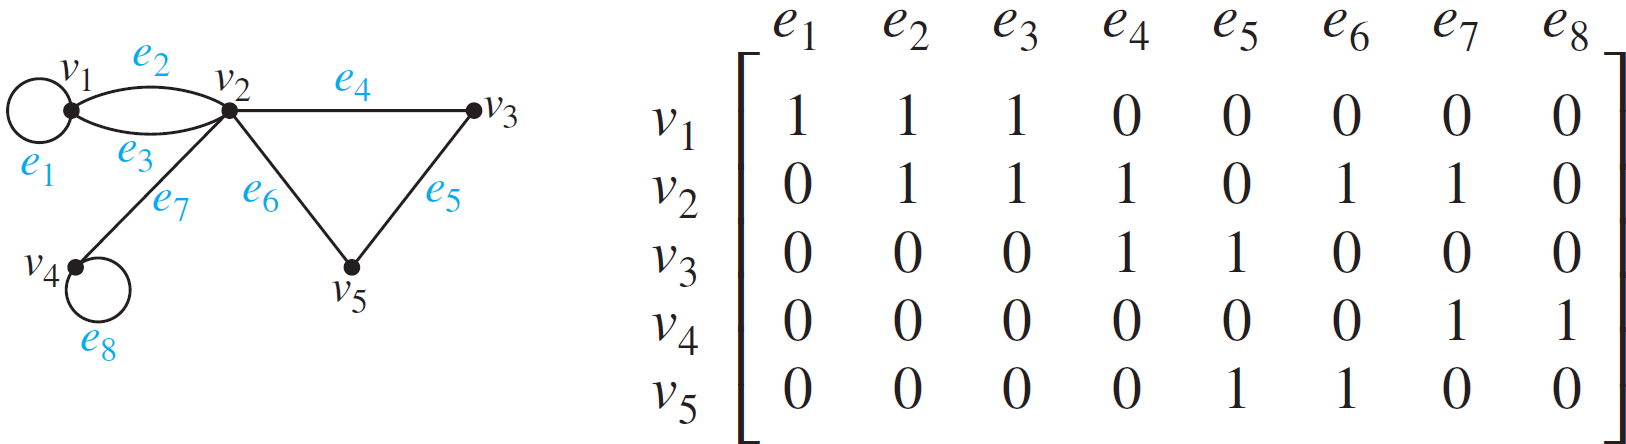
\includegraphics[width=.75\textwidth]{img/ch10.3-figure7.png}
    \label{fig:my_label}
\end{figure}

\subsection{Isomorphism of Graphs}

We often need to know whether it is possible to draw two graphs in the same way. That is, do the graphs have the same structure when we ignore the identities of their vertices? For instance, in chemistry, graphs are used to model chemical compounds. Different compounds can have the same molecular formula but can differ in structure. Such compounds can be represented by graphs that cannot be drawn in the same way. The graphs representing previously known compounds can be used to determine whether a supposedly new compound has been studied before. There is a useful terminology for graphs with the same structure.

\begin{definition}{1}
The simple graphs $G_1 = (V_1,\ E_1)$ and $G_2 = (V_2,\ E_2)$ are \textit{isomorphic} if there exists a one-to-one and onto function $f$ from $V_1$ to $V_2$ with the property that $a$ and $b$ are adjacent in $G_1$ if and only if $f(a)$ and $f(b)$ are adjacent in $G_2$, for all $a$ and $b$ in $V_1$. Such a function $f$ is called an \textbf{\textit{isomorphism}}.$^{*}$ Two simple graphs that are not isomorphic are called \textbf{\textit{nonisomorphic}}.
\end{definition}

In other words, when two simple graphs are isomorphic, there is a one-to-one correspondence between vertices of the two graphs that preserves the adjacency relationship. Isomorphism of simple graphs is an equivalence relation. \textit{(Check Example 8 in Chapter 10.3 in text book)}

\begin{mybox}{violet}{The number of Isomorphic Graphs}
If there are $n$ vertices in a graph, there are $n!$ isomorphic graphs having the same set of vertices.
\end{mybox}

\subsection{Determining whether Two Simple Graphs are Isomorphic}

It is often difficult to determine whether two simple graphs are isomorphic or not. There are $n!$ possible one-to-one correspondences between the vertex sets of two simple graphs with $n$ vertices. Testing each such correspondence to see whether it preserves adjacency and nonadjacency is impractical if $n$ is at all large.

Sometimes it is not hard to show that two graphs are not isomorphic. In particular, we can show that two graphs are not isomorphic if we can find a property only one of the two graphs has, but that is preserved by isomorphism. A property preserved by isomorphism of graphs is called a \textbf{graph invariant}. For instance, isomorphic simple graphs must have the same number of vertices, because there is a one-to-one correspondence between the sets of vertices of the graphs.

Isomorphic simple graphs also must have the same number of edges, because the one-to-one correspondence between vertices establishes a one-to-one correspondence between edges. In addition, the degrees of the vertices in isomorphic simple graphs must be the same. That is, a vertex $v$ of degree $d$ in $G$ must correspond to a vertex $f(v)$ of degree $d$ in $H$, because a vertex
$w$ in $G$ is adjacent to $v$ if and only if $f(v)$ and $f(w)$ are adjacent in $H$.

\textit{The number of vertices, the number of edges, and the number of vertices of each degree are all invariants under isomorphism}. If any of these quantities differ in two simple graphs, these graphs \textit{cannot be isomorphic}. However, when these invariants are the same, it does not necessarily mean that the two graphs are isomorphic. There are no useful sets of invariants currently known that can be used to determine whether simple graphs are isomorphic.

To show that a function $f$ from the vertex set of a graph $G$ to the vertex set of a graph $H$ is an isomorphism, we need to show that $f$ \textit{preserves the presence and absence of edges}. One helpful way to do this is to use adjacency matrices. 

In particular, to show that $f$ is an isomorphism, we can show that the adjacency matrix of $G$ is the same as the adjacency matrix of $H$, when rows and columns are labeled to correspond to the images under $f$ of the vertices in $G$ that are the labels of these rows and columns in the adjacency matrix of $G$.

\textit{("Algorithms For Graph Isomorphism" and "Applications Of Graph Isomorphisms" should be read from text book)}


\section{Connectivity}

\subsection{Introduction}

Many problems can be modeled with paths formed by traveling along the edges of graphs. For instance, the problem of determining whether a message can be sent between two computers using intermediate links can be studied with a graph model. Problems of efficiently planning routes for mail delivery, garbage pickup, diagnostics in computer networks, and so on can be solved using models that involve paths in graphs.

\subsection{Paths}

Informally, a \textbf{path} is a sequence of edges that begins at a vertex of a graph and travels from vertex to vertex along edges of the graph. As the path travels along its edges, it visits the vertices along this path, that is, the endpoints of these edges.

A formal definition of paths and related terminology is given in Definition 1.

\begin{definition}{1}
Let $n$ be a nonnegative integer and $G$ an undirected graph. A \textit{path} of \textit{length $n$} from $u$ to $v$ in $G$ is a sequence of $n$ edges $e_1, ..., e_n$ of $G$ for which there exists a sequence $x_0 = u$, $x_1$, ..., $x_{n-1}$, $x_n = v$ of vertices such that $e_i$ has, for $i = 1, ..., n$, the endpoints $x_{i-1}$ and $x_i$. When the graph is simple, we denote this path by its vertex sequence $x_0, x_1, ..., x_n$ (because listing these vertices uniquely determines the path).

The path is a \textbf{circuit} if it \textit{begins and ends at the same vertex}, that is, if $u = v$, and has length greater than zero. The path or circuit is said to pass through the vertices $x_1, x_2, ..., x_{n-1}$ or traverse the edges $e_1, e_2, ..., e_n$. A path or circuit is simple if it does not contain the same edge more than once.
\end{definition}

\newpage
\textbf{Remark:} There is considerable variation of terminology concerning the concepts defined in Definition 1. For instance, in some books, the term \textbf{walk} is used instead of \textit{\textbf{path}}, where a walk is defined to be an alternating sequence of vertices and edges of a graph, $v_0, e_1, v_1, e_2, ..., v_{n-1}, e_n, v_n$, where $v_i - 1$ and $v_i$ are the endpoints of $e_i$ for $i = 1, 2, ..., n$. When this terminology is used, \textbf{closed walk} is used instead of \textit{\textbf{circuit}} to indicate a walk that begins and ends at the same vertex, and \textbf{trail} is used to denote \textit{a walk that has no repeated edge} (replacing the term \textit{\textbf{simple path}}). When this terminology is used, the terminology \textbf{path} is often used for a \textit{\textbf{trail}} with no repeated vertices, conflicting with the terminology in Definition 1. Because of this variation in terminology, you will need to make sure which set of definitions are used in a particular book or article when you read about traversing edges of a graph.

\begin{definition}{2}
Let $n$ be a nonnegative integer and $G$ a directed graph. A \textit{path} of length $n$ from $u$ to $v$ in $G$ is a sequence of edges $e_1, e_2, ..., e_n$ of $G$ such that $e_1$ is associated with $(x_0, x_1)$, $e_2$ is associated with $(x_1, x_2)$, and so on, with $e_n$ associated with $(x_{n-1}, x_n)$, where $x_0 = u$ and $x_n = v$. When there are no multiple edges in the directed graph, this path is denoted by its vertex sequence $x_0, x_1, x_2, ..., x_n$. A path of length greater than zero that begins and ends at the same vertex is called a \textbf{circuit} or \textbf{cycle}. A \textit{path} or \textit{circuit} is called \textbf{simple} if it does not contain the same edge more than once.
\end{definition}

\noindent \textbf{Remark:} Terminology other than that given in Definition 2 is often used for the concepts defined there. In particular, the alternative terminology that uses walk, closed walk, trail, and path.

Note that the terminal vertex of an edge in a path is the initial vertex of the next edge in the path. When it is not necessary to distinguish between multiple edges, we will denote a path $e_1, e_2, ..., e_n$, where $e_i$ is associated with $(x_{i-1}, x_i)$ for $i = 1, 2, ..., n$, by its vertex sequence $x_0, x_1, ..., x_n$. The notation identifies a path only as far as which the vertices it passes through. There may be more than one path that passes through this sequence of vertices, which will happen if and only if there are multiple edges between two successive vertices in the list.

\subsection{Connectedness in Undirected Graphs}

\begin{definition}{3}
An undirected graph is called \textit{\textbf{connected}} if there is a path between every pair of distinct vertices of the graph. An undirected graph that is not connected is called \textit{\textbf{disconnected}}. We say that we disconnect a graph when we remove vertices or edges, or both, to produce a disconnected subgraph.
\end{definition}

\begin{theorem}{1}
There is a simple path between every pair of distinct vertices of a connected undirected graph.
\end{theorem}

\subsubsection{Connected Components}

A \textbf{connected component} of a graph $G$ is a connected subgraph of $G$ that is not a proper subgraph of another connected subgraph of $G$. That is, a connected component of a graph $G$ is a maximal connected subgraph of $G$. A graph $G$ that is not connected has two or more connected components that are disjoint and have $G$ as their union.

\newpage
\subsection{How Connected is a Graph?}

Sometimes the removal from a graph of a vertex and all incident edges produces a subgraph with more connected components. Such vertices are called \textbf{cut vertices} (or \textbf{articulation points}). The removal of a cut vertex from a connected graph produces a subgraph that is not connected. Analogously, an edge whose removal produces a graph with more connected components than in the original graph is called a \textbf{cut edge} or \textbf{bridge}.

\subsubsection{Vertex Connectivity}

Not all graphs have cut vertices. For example, the complete graph $K_n$, where $n \geq 3$, has no cut vertices. When you remove a vertex from $K_n$ and all edges incident to it, the resulting subgraph is the complete graph $K_{n-1}$, a connected graph. Connected graphs without cut vertices are called \textbf{nonseparable graphs}, and can be thought of as more connected than those with a cut vertex. We can extend this notion by defining a more granulated measure of graph connectivity based on the minimum number of vertices that can be removed to disconnect a graph.

A subset $V^{'}$ of the vertex set $V$ of $G = (V,\ E)$ is a \textbf{vertex cut}, or \textbf{separating set}, if $G - V^{'}$ is disconnected. Every connected graph, except a complete graph, has a vertex cut. We define the \textbf{vertex connectivity} of a noncomplete graph $G$, denoted by $\kappa(G)$, as the minimum number of vertices in a vertex cut.

When $G$ is a complete graph, it has no vertex cuts, because removing any subset of its vertices and all incident edges still leaves a complete graph. Consequently, we cannot define $\kappa(G)$ as the minimum number of vertices in a vertex cut when $G$ is complete. Instead, we set $\kappa(K_n) = n - 1$, the number of vertices needed to be removed to produce a graph with a single vertex.

Consequently, for every graph $G$, $\kappa(G)$ is minimum number of vertices that can be removed from G to either disconnect $G$ or produce a graph with a single vertex. We have $0 \leq \kappa(G) \leq n-1$ if $G$ has $n$ vertices, $\kappa(G) = 0$ if and only if $G$ is disconnected or $G = K_1$ and $\kappa(G) = n-1$ if and only if $G$ is complete.

The larger $\kappa(G)$ is, the more connected we consider $G$ to be. Disconnected graphs and $K_1$ have $\kappa(G) = 0$, connected graphs with cut vertices and $K_2$ have $\kappa(G) = 1$, graphs without cut vertices that can be disconnected by removing two vertices and $K_3$ have $\kappa(G) = 2$, and so on.

We say that a graph is \textbf{$k$-connected} (or \textbf{$k$-vertex-connected}), if $\kappa(G) \geq k$. A graph $G$ is 1-connected if it is connected and not a graph containing a single vertex; a graph is 2-connected, or \textbf{biconnected}, if it is nonseparable and has at least three vertices. Note that if $G$ is a k-connected graph, then $G$ is a $j$-connected graph for all $j$ with $0 \leq j \leq k$.

\subsubsection{Edge Connectivity}

We can also measure the connectivity of a connected graph $G = (V, E)$ in terms of the minimum number of edges that we can remove to disconnect it. If a graph
has a cut edge, then we need only remove it to disconnect $G$. If $G$ does not have a cut edge, we look for the smallest set of edges that can be removed to disconnect it. A set of edges $E^{'}$ is called an \textbf{edge cut} of $G$ if the subgraph $G - E^{'}$ is disconnected. The \textbf{edge connectivity} of a graph $G$, denoted by $\lambda(G)$, is the minimum number of edges in an edge cut of $G$. 

This defines $\lambda(G)$ for all connected graphs with more than one vertex because it is always possible to disconnect such a graph by removing all edges incident to one of its vertices. 

Note that $\lambda(G) = 0$ if $G$ is not connected. We also specify that $\lambda(G) = 0$ if $G$ is a graph consisting of a single vertex. It follows that if $G$ is a graph with $n$ vertices, then $0 \leq \lambda(G) \leq n-1$. $\lambda(G) = n-1$ where $G$ is a graph with $n$ vertices if and only if
$G = K_n$, which is equivalent to the statement that $\lambda(G) \leq n-2$ when $G$ is not a complete graph.

\subsubsection{An Inequality For Vertex Connectivity And Edge Connectivity}

When $G = (V, E)$ is a noncomplete connected graph with at least three vertices, the minimum degree of a vertex of $G$ is an upper bound for both the vertex connectivity of $G$ and the edge connectivity of $G$. That is, $\kappa(G) \leq min_{v \in V} deg(v)$ and $\lambda(G) \leq min_{v \in V} deg(v)$. 

To see this, observe that deleting all the neighbors of a fixed vertex of minimum degree disconnects $G$, and deleting all the edges that have a fixed vertex of minimum degree as an endpoint disconnects $G$.

$\kappa(G) \leq \lambda(G)$ when $G$ is a connected noncomplete graph. Note also that $\kappa(K_n) = \lambda(K_n) = min_{v \in V} deg(v) = n-1$ when $n$ is a positive integer and that $\kappa(G) = \lambda(G) = 0$ when $G$ is a disconnected graph. Putting these facts together establishes that for all graphs $G$,

$ \kappa(G) \leq \lambda(G) \leq min_{v \in V} deg(v) $

\subsubsection{Applications Of Vertex And Edge Connectivity}

\textit{(This little part should be read from text book)}

\subsection{Connectedness in Directed Graphs}

There are two notions of connectedness in directed graphs, depending on whether the directions of the edges are considered.

\begin{definition}{4}
A directed graph is \textit{\textbf{strongly connected}} if there is a path from $a$ to $b$ and from $b$ to $a$ whenever $a$ and $b$ are vertices in the graph.
\end{definition}

For a directed graph to be strongly connected there must be a sequence of directed edges from any vertex in the graph to any other vertex. A directed graph can fail to be strongly connected but still be in “one piece.” Definition 5 makes this notion precise.

\begin{definition}{5}
A directed graph is \textit{\textbf{weakly connected}} if there is a path between every two vertices in the underlying undirected graph.
\end{definition}

That is, a directed graph is weakly connected if and only if there is always a path between two vertices when the directions of the edges are disregarded. Clearly, any strongly connected directed graph is also weakly connected.

\subsubsection{Strong Components Of A Directed Graph}

The subgraphs of a directed graph $G$ that are strongly connected but not contained in larger strongly connected subgraphs, that is, the maximal strongly connected subgraphs, are called the \textbf{strongly connected components} or \textbf{strong components} of $G$. Note that if $a$ and $b$ are two vertices in a directed graph, their strong components are either the same or disjoint.

\subsection{Paths and Isomorphism}

There are several ways that paths and circuits can help determine whether two graphs are isomorphic. For example, the existence of a simple circuit of a particular length is a useful invariant that can be used to show that two graphs are not isomorphic. In addition, paths can be used to construct mappings that may be isomorphisms.

As we mentioned, a useful isomorphic invariant for simple graphs is the existence of a simple circuit of length $k$, where $k$ is a positive integer greater than 2. \textit{(Examples of this part should be read.)}

\subsection{Counting Paths Between Vertices}

The number of paths between two vertices in a graph can be determined using its adjacency matrix.

\begin{theorem}{2}
Let $G$ be a graph with adjacency matrix $A$ with respect to the ordering $v_1, v_2, ..., v_n$ of the vertices of the graph (with directed or undirected edges, with multiple edges and loops allowed). The number of different paths of length $r$ from $v_i$ to $v_j$, where $r$ is a positive integer, equals the $(i, j)^{th}$ entry of $A^r$.
\end{theorem}

\textbf{Proof:} The theorem will be proved using mathematical induction. Let $G$ be a graph with adjacency matrix $A$ (assuming an ordering $v_1, v_2, ..., v_n$ of the vertices of $G$). The number of paths from $v_i$ to $v_j$ of length $1$ is the $(i, j)^{th}$ entry of $A$, because this entry is the number of edges from $v_i$ to $v_j$.

Assume that the $(i, j)^{th}$ entry of $A^r$ is the number of different paths of length $r$ from $v_i$ to $v_j$. This is the inductive hypothesis. Because $A^{r+1} = A^{r}A$, the $(i, j)^{th}$ entry of $A^{r+1}$ equals

$b_{i1}a{1j} + b_{i2}a_{2j} + \cdot \cdot \cdot + b_{in}a_{nj}$

\noindent where $b_{ik}$ is the $(i, k)^{th}$ entry of $A^r$. By the inductive hypothesis, $b_{ik}$ is the number of paths of length $r$ from $v_i$ to $v_k$.

A path of length $r + 1$ from $v_i$ to $v_j$ is made up of a path of length $r$ from $v_i$ to some intermediate vertex $v_k$, and an edge from $v_k$ to $v_j$. By the product rule for counting, the number of such paths is the product of the number of paths of length $r$ from $v_i$ to $v_k$, namely, $b_{ik}$, and the number of edges from $v_k$ to $v_j$, namely, $a_{kj}$. When these products are added for all possible intermediate vertices $v_k$, the desired result follows by the sum rule for counting.

Theorem 2 can be used to find the length of the shortest path between two vertices of a graph, and it can also be used to determine whether a graph is connected.

\section{Euler and Hamilton Paths}

\subsection{Introduction}

Can we travel along the edges of a graph starting at a vertex and returning to it by traversing each edge of the graph exactly once? Similarly, can we travel along the edges of a graph starting at a vertex and returning to it while visiting each vertex of the graph exactly once? Although these questions seem to be similar, the first question, which asks whether a graph has an \textit{Euler circuit}, can be easily answered simply by examining the degrees of the vertices of the graph, while the second question, which asks whether a graph has a \textit{Hamilton circuit}, is quite difficult to solve for most graphs. In this section we will study these questions and discuss the difficulty of solving them. Although both questions have many practical applications in many different areas, both arose in old puzzles. We will learn about these old puzzles as well as modern practical applications.

\subsection{Euler Paths and Circuits}

An \textbf{Euler path} is a path that uses every edge of a graph exactly once.\\
An \textbf{Euler circuit} is a circuit that uses every edge of a graph exactly 
once.
\begin{itemize}
    \item An Euler path starts and ends at \textit{different} vertices.
    \item An Euler circuit starts and ends at \textit{the same} vertex.
\end{itemize}

\subsubsection{The Criterion for Euler Paths}

Suppose that a graph has an Euler path $P$. For every vertex $v$ other than the starting and ending vertices, the path $P$ \textit{enters} $v$ \textbf{the same number of times} that it \textit{leaves} $v$ (say $s$ times).

Therefore, there are $2s$ edges having $v$ as an endpoint. Therefore, all vertices other than the two endpoints of $P$ must be even vertices.

Suppose the Euler path $P$ starts at vertex $x$ and ends at $y$. Then $P$ \textit{leaves $x$ one more time than it enters}, and \textit{leaves $y$
one fewer time than it enters}. 

Therefore, the two endpoints of $P$ must be \textbf{odd vertices}.

The inescapable conclusion ("based on reason alone!"):
\begin{mybox}{violet}{Criteria of Euler Path}
If a graph $G$ has an Euler path, then it must have \textit{exactly} two odd vertices.\\

Or, to put it another way,\\

If the number of odd vertices in $G$ is anything other than 2, then $G$ cannot have an Euler path.
\end{mybox}

\subsubsection{The Criterion for Euler Circuits}

Suppose that a graph $G$ has an Euler circuit $C$. For every vertex $v$ in $G$, each edge having $v$ as an endpoint shows up exactly once in $C$. The circuit $C$ \textit{enters $v$ \textbf{the same number of times} that it
leaves $v$ (say $s$ times)}, so $v$ has degree $2s$. That is, \textit{$v$ must be an \textbf{even vertex}.}

The inescapable conclusion ("based on reason alone"):
\begin{mybox}{violet}{Criteria of Euler Circuit}
If a graph $G$ has an Euler circuit, then all of its vertices must be even vertices.\\

Or, to put it another way,\\

If the number of odd vertices in $G$ is anything other than 0, then $G$ cannot have an Euler circuit.
\end{mybox}

\begin{table}[h!]
    \centering
    \begin{tabular}{|c|c|c|}
        \hline
        \# of odd vertices & Eular path & Euler Circuit \\ \hline
        0 & No & Maybe \\ \hline
        2 & Maybe & No \\ \hline
        4, 6, 8, ... & No & No \\ \hline
        1, 3, 5, ... & No such graph & No such graph \\ \hline
    \end{tabular}
\end{table}

When, *provided the graph is connected.

\begin{table}[h!]
    \centering
    \begin{tabular}{|c|c|c|}
        \hline
        \# of odd vertices & Eular path & Euler Circuit \\ \hline
        0 & No & Yes* \\ \hline
        2 & Yes* & No \\ \hline
        4, 6, 8, ... & No & No \\ \hline
        1, 3, 5, ... & No such graph & No such graph \\ \hline
    \end{tabular}
\end{table}

\newpage
\subsubsection{Finding Euler Circuits and Paths}

To find an Euler path or an Euler circuit:
\begin{enumerate}
    \item Make sure the graph has either 0 or 2 odd vertices.
    \item If there are 0 odd vertices, start anywhere. If there are 2 odd vertices, start at one of them.
    \item Follow edges one at a time. If you have a choice between a bridge and a non-bridge, always choose the non-bridge.
    \item Stop when you run out of edges.
\end{enumerate}

This is called \textbf{Fleury's algorithm}, and it always works!

\subsection{Hamilton Paths and Circuits}

A \textbf{Hamilton Path} is a path that goes through \textit{every vertex} of a graph exactly once.\\
A \textbf{Hamilton Circuit} is a Hamilton Path that \textit{begins and ends at the same vertex}.

\textbf{Important:} In here, there is no need to be used all the edges. Unlike Euler Paths and Circuits, there is no trick to tell if a graph has a Hamilton Path or Circuit.

\subsubsection{Conditions For The Existence Of Hamilton Circuits}

Is there a simple way to determine whether a graph has a Hamilton circuit or path? At first, it might seem that there should be an easy way to determine this, because there is a simple way to answer the similar question of whether a graph has an Euler circuit. Surprisingly, there are no known simple necessary and sufficient criteria for the existence of Hamilton circuits.

However, many theorems are known that give sufficient conditions for the existence of Hamilton circuits. Also, certain properties can be used to show that a graph has no Hamilton circuit. 

For instance, a graph with a vertex of degree one cannot have a Hamilton circuit, because in a Hamilton circuit, each vertex is incident with two edges in the circuit. Moreover, if a vertex in the graph has degree two, then both edges that are incident with this vertex must be part of any Hamilton circuit. 

Also, note that when a Hamilton circuit is being constructed and this circuit has passed through a vertex, then all remaining edges incident with this vertex, other than the two used in the circuit, can be removed from consideration. Furthermore, a Hamilton circuit cannot contain a smaller circuit within it.\\


Although no useful necessary and sufficient conditions for the existence of Hamilton circuits are known, quite a few sufficient conditions have been found. Note that the more edges a graph has, the more likely it is to have a Hamilton circuit. Furthermore, adding edges (but not vertices) to a graph with a Hamilton circuit produces a graph with the same Hamilton circuit.

So as we add edges to a graph, especially when we make sure to add edges to each vertex, we make it increasingly likely that a Hamilton circuit exists in this graph. Consequently, we would expect there to be sufficient conditions for the existence of Hamilton circuits that depend on the degrees of vertices being sufficiently large. We state two of the most important sufficient conditions here. These conditions were found by Gabriel A. Dirac in 1952 and $\centernot{O}$ystein Ore in 1960.

\begin{theorem}{DIRAC’S THEOREM}
If $G$ is a simple graph with $n$ vertices with $n \geq 3$ such that the degree of every vertex in $G$ is at least $n/2$, then $G$ has a Hamilton circuit.
\end{theorem}

\begin{theorem}{ORE’S THEOREM}
If $G$ is a simple graph with $n$ vertices with $n \geq 3$ such that $deg(u) + deg(v) \geq n$ for every pair of nonadjacent vertices $u$ and $v$ in $G$, then $G$ has a Hamilton circuit.
\end{theorem}

\begin{theorem}{}
Let the number of edges of $G$ be $m$. Then $G$ has a Hamilton circuit if $m \geq \frac{n^2-3n+6}{2}$ where $n$ is the number of vertices.
\end{theorem}

The number of Hamilton circuits in a complete graph with $n$ vertices, including reversals, is equal to $(n-1)!$ If reversals are not included, the number of Hamilton circuits becomes $\frac{(n-1)!}{2}$.

\section{Shortest-Path}

\textit{(This part may be read from the text book)}.

\section{Planar Graphs}

\subsection{Introduction}

\begin{definition}{1}
A graph is called \textit{\textbf{planar}} if it can be drawn in the plane without any edges crossing (where a crossing of edges is the intersection of the lines or arcs representing them at a point other than their common endpoint). Such a drawing is called a \textit{\textbf{planar representation} of the graph}.
\end{definition}

\subsection{Euler’s Formula}

\begin{wrapfigure}{r}{0.3\textwidth}
    \centering
    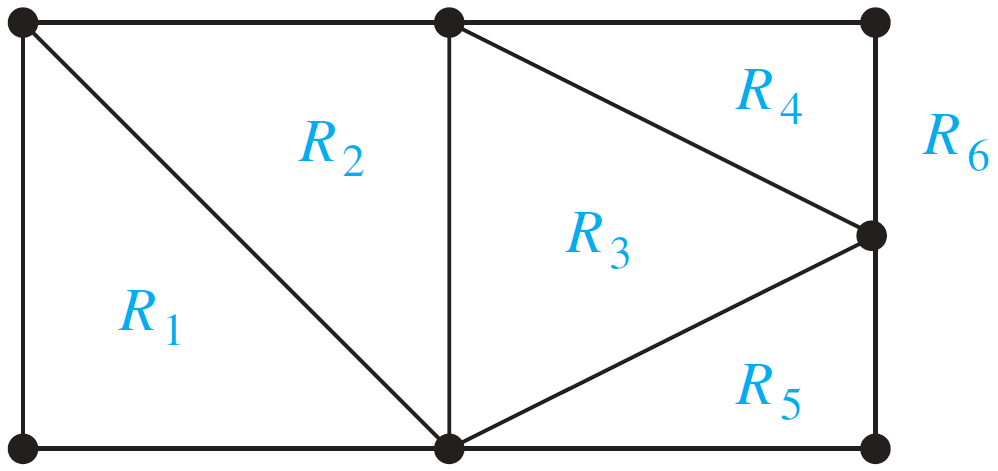
\includegraphics[width=0.3\textwidth]{img/ch10.7-figure8.png}
    \caption{The regions of the planar representation of a graph.}
\end{wrapfigure}

A planar representation of a graph splits the plane into regions, including an unbounded region. For instance, the planar representation of the graph shown in Figure 3 splits the plane into six regions. These are labeled in the figure. 

Euler showed that all planar representations of a graph split the plane into the same number of regions. He accomplished this by finding a relationship among the number of regions, the number of vertices, and the number of edges of a planar graph.

\begin{mybox}{violet}{\textbf{EULER’S FORMULA}}
Let $G$ be a connected planar simple graph with $e$ edges and $v$ vertices. Let $r$ be the number of regions in a planar representation of $G$. Then $r = e - v + 2$.
\end{mybox}

\textit{(Proof of the Euler's Formula can be found in the text book)}.\\

Euler’s formula can be used to establish some inequalities that must be satisfied by planar graphs. One such inequality is given in Corollary 1.

\begin{mybox}{violet}{\textbf{Corollary 1}}
If $G$ is a connected planar simple graph with $e$ edges and $v$ vertices, where $v \geq 3$, then $e \leq 3v - 6$.
\end{mybox}

\begin{mybox}{violet}{\textbf{Corollary 2}}
If $G$ is a connected planar simple graph, then $G$ has a vertex of degree not exceeding five.
\end{mybox}

\textit{(Proof of the Corollary 1 and Corollary 2 can be found in the text book)}.

The proof of Corollary 1 is based on the concept of the \textbf{degree} of a region, which is defined to be the number of edges on the boundary of this region. When an edge occurs twice on the boundary (so that it is traced out twice when the boundary is traced out), it contributes two to the degree. We denote the degree of a region $R$ by $deg(R)$.

\begin{mybox}{violet}{\textbf{Corollary 3}}
If a connected planar simple graph has $e$ edges and $v$ vertices with $v \geq 3$ and no circuits of length three, then $e \leq 2v - 4$.
\end{mybox}

\subsection{Kuratowski’s Theorem}

A graph is not planar if it contains either of these two graphs as a subgraph. Surprisingly, all nonplanar graphs must contain a subgraph that can be obtained from $K_{3,3}$ or $K_5$ using certain permitted operations.

If a graph is planar, so will be any graph obtained by removing an edge $\{u, v\}$ and adding a new vertex $w$ together with edges $\{u, w\}$ and $\{w, v\}$. Such an operation is called an \textbf{elementary subdivision}. The graphs $G_1 = (V_1, E_1)$ and $G_2 = (V_2, E_2)$ are called \textbf{homeomorphic} if they can be obtained from the same graph by a sequence of elementary subdivisions.

\begin{theorem}{2}
A graph is nonplanar if and only if it contains a subgraph homeomorphic to $K_{3,3}$ or $K_5$.
\end{theorem}

\section{Graph Coloring}

\begin{definition}{1}
A \textit{\textbf{coloring}} of a simple graph is the assignment of a color to each vertex of the graph so that no two adjacent vertices are assigned the same color.
\end{definition}

\begin{definition}{2}
The \textit{\textbf{chromatic number}} of a graph is the least number of colors needed for a coloring of this graph. The chromatic number of a graph $G$ is denoted by $\chi(G)$.
\end{definition}

Note that asking for the chromatic number of a planar graph is the same as asking for the minimum number of colors required to color a planar map so that no two adjacent regions are assigned the same color.

\begin{theorem}{1: The Four Color Theorem}
The chromatic number of a planar graph is no greater than four.
\end{theorem}

\textit{(It is better idea to read this part from the text book.)}

\subsection{Applications of Graph Colorings}

\textit{(It is better idea to read this part from the text book.)}

\end{document}
